\chapter{Empirical Analysis}
\label{chap:empirical_analysis}

Generally, in the sources that have been leaked, a gradually increasing number of incorporations. Entity creation across different data leaks. Figure \ref{fig:incorporations_time} illustrates the number of entity incorporations over time, segmented by the source investigation (e.g., Panama Papers, Pandora Papers).

\begin{figure}[htbp]
    \centering
    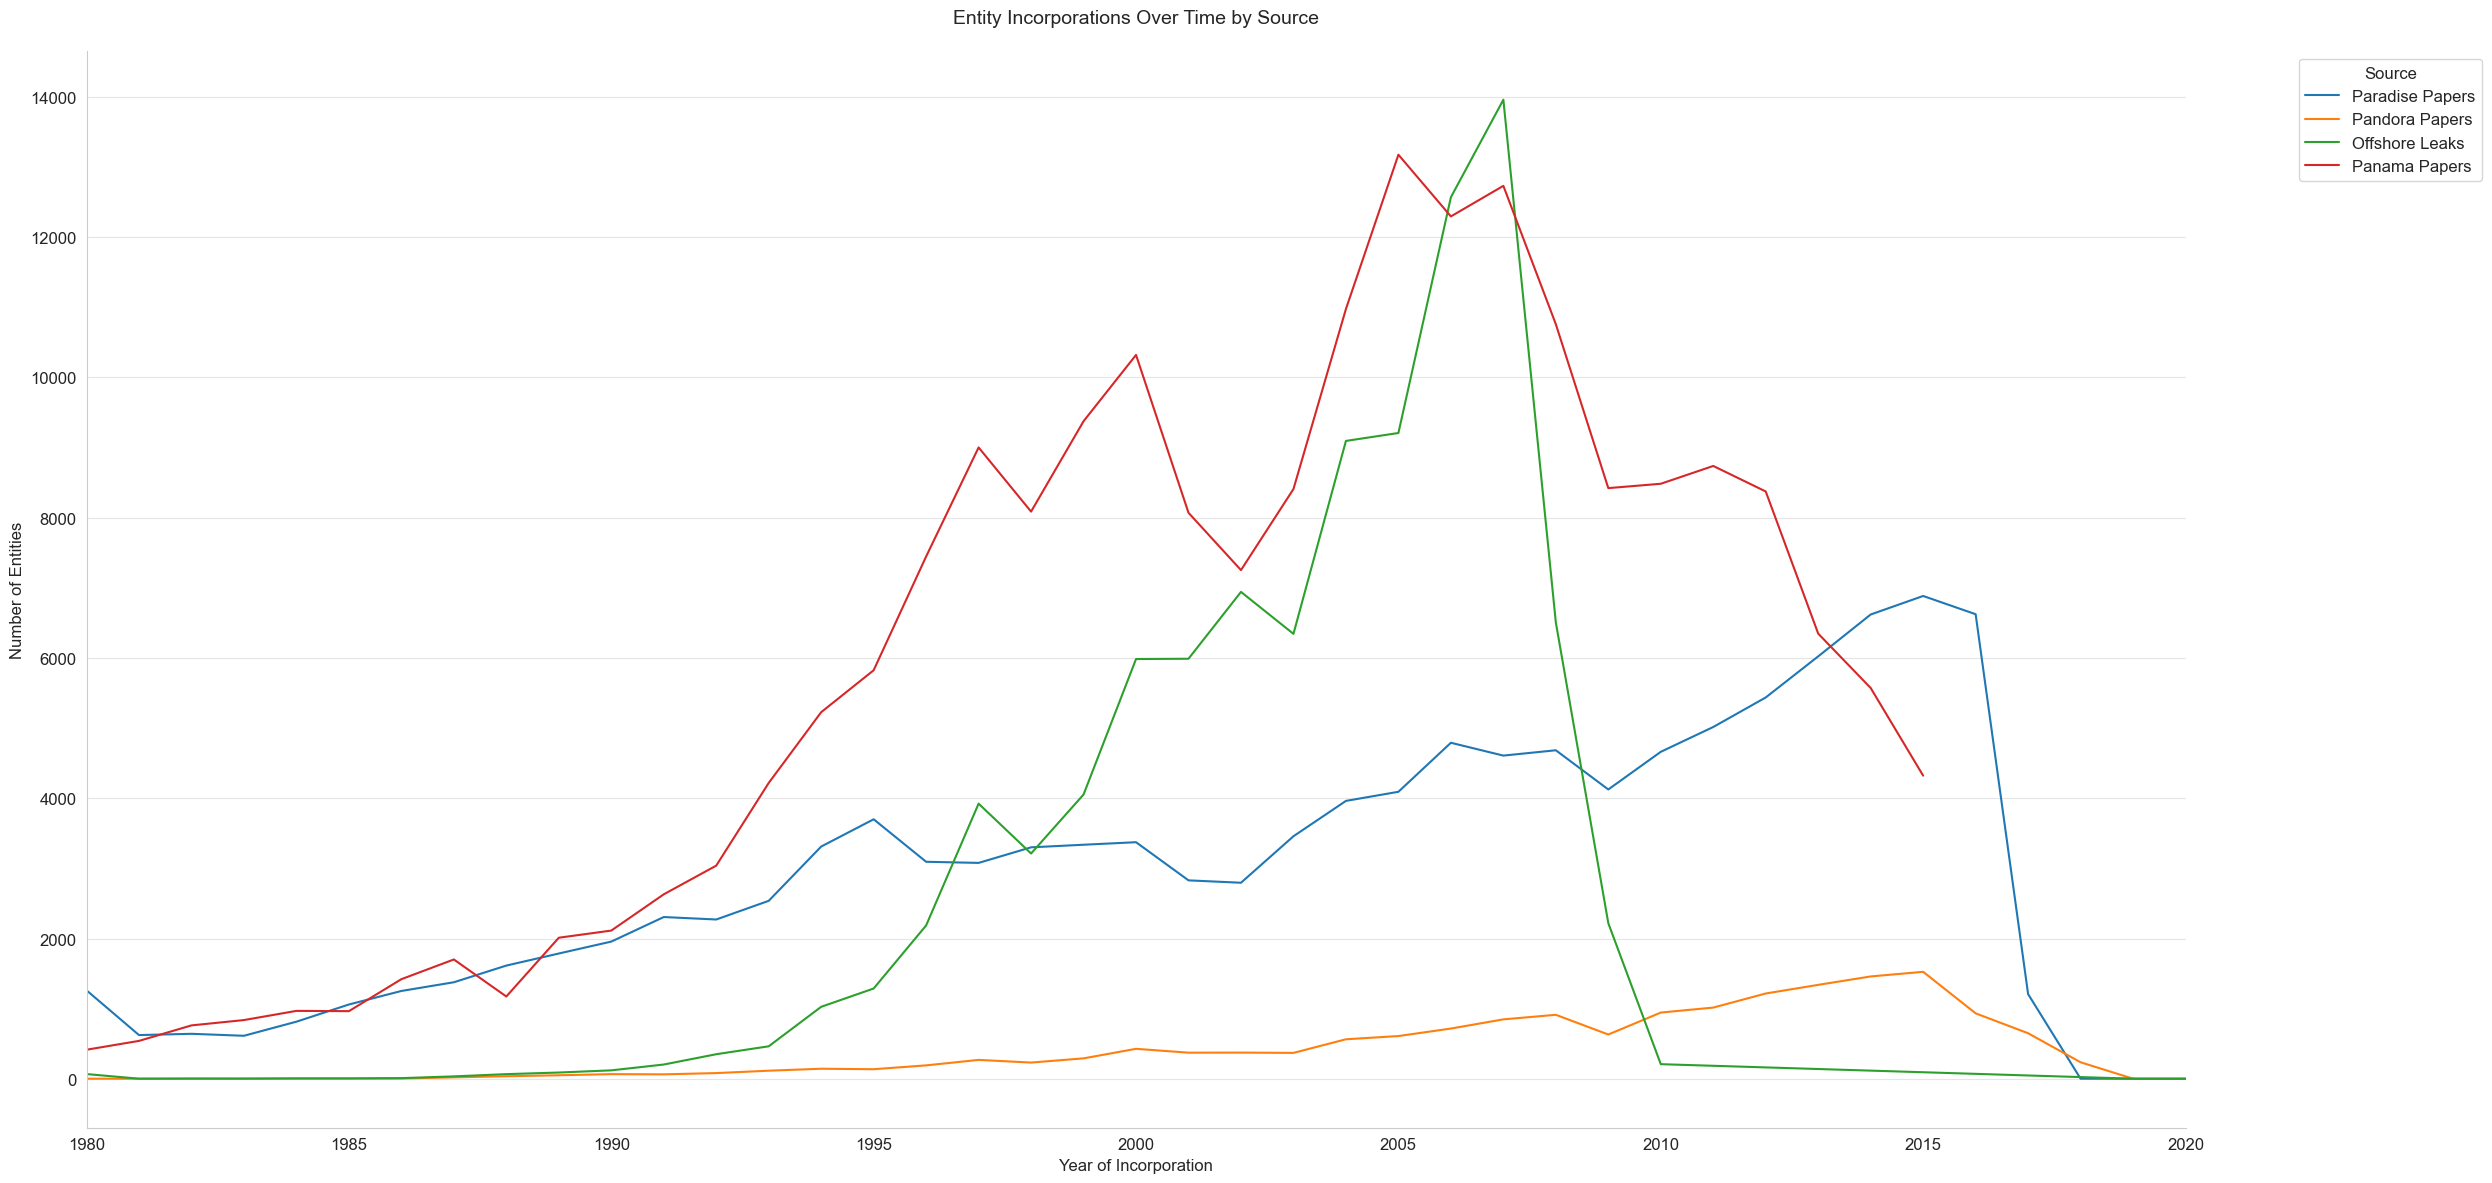
\includegraphics[width=0.8\textwidth]{incorporationsovertime.png}
    \caption{Entity Incorporations Over Time by Source Investigation.}
    \label{fig:incorporations_time}
\end{figure}

Because of the power-law distribution intermediaries follow in terms of their connections (see Figure \ref{fig:powerlaw_dist}), we can explain a significant portion of the network activity by enriching the top fraction of intermediaries. Specifically, enriching the top approximately 750 intermediaries (ranked by the number of entities they are connected to) provides substantial coverage of ~60\% entities, as shown in Figure \ref{fig:enrichment_coverage_pie}.

\begin{figure}[htbp]
    \centering
    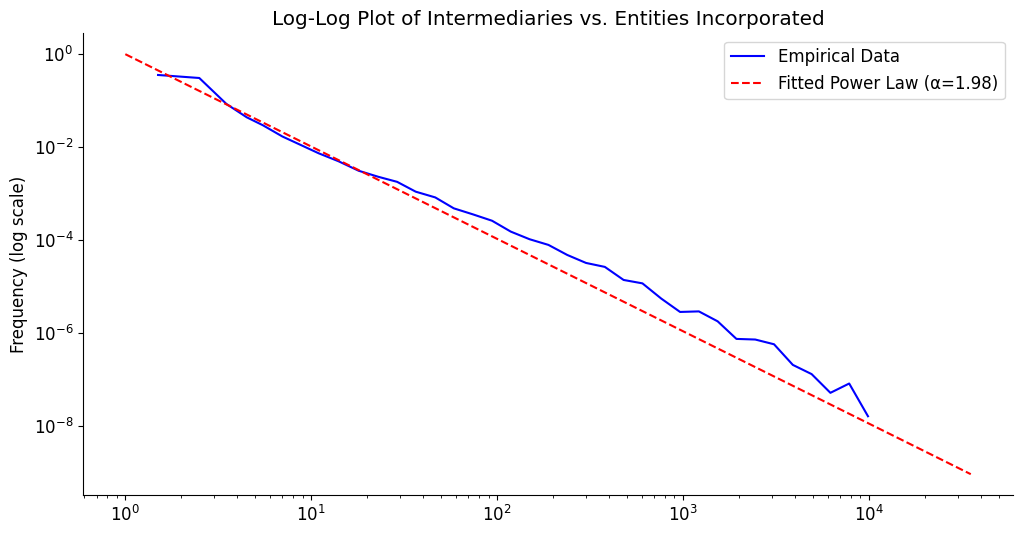
\includegraphics[width=0.8\textwidth]{powerlaw.png}
    \caption{Illustration of the Power Law Distribution of Intermediary Connections (Degree).}
    \label{fig:powerlaw_dist}
\end{figure}

\begin{figure}[htbp]
    \centering
    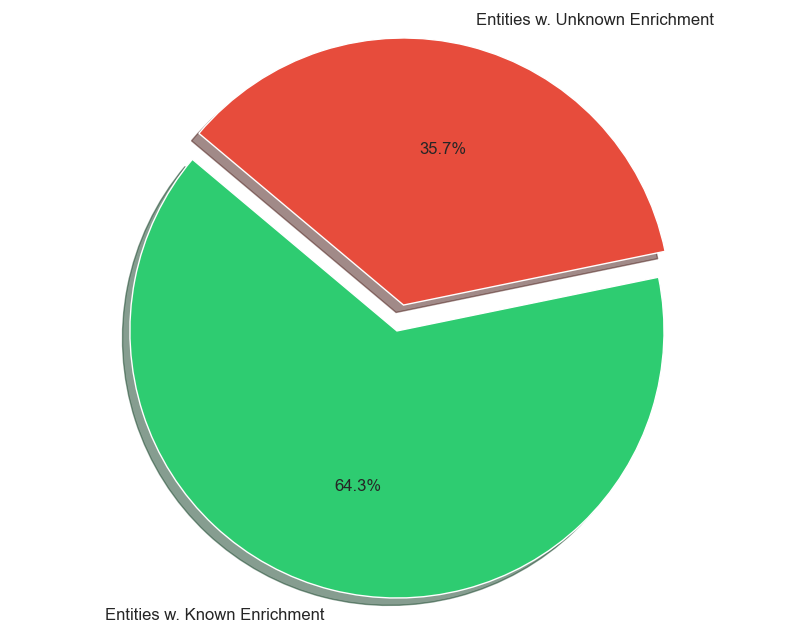
\includegraphics[width=0.8\textwidth]{piechartenrichment.png}
    \caption{Coverage of Intermediary Connections Explained by the Enriched Top Intermediaries.}
    \label{fig:enrichment_coverage_pie}
\end{figure}

The geographic distribution and coverage of different node types (intermediaries, entities, officers) provide further context. Figures \ref{fig:int_locations} and \ref{fig:int_coverage} show the primary locations of intermediaries and the coverage achieved by focusing on the top locations. Similarly, Figures \ref{fig:ent_locations} and \ref{fig:ent_coverage} depict the distribution and coverage for entities, while Figures \ref{fig:off_locations} and \ref{fig:off_coverage} do the same for officers.

The common thread across all of them, is that all are incredibly concentrated in a limited number of countries.

\begin{figure}[htbp]
    \centering
    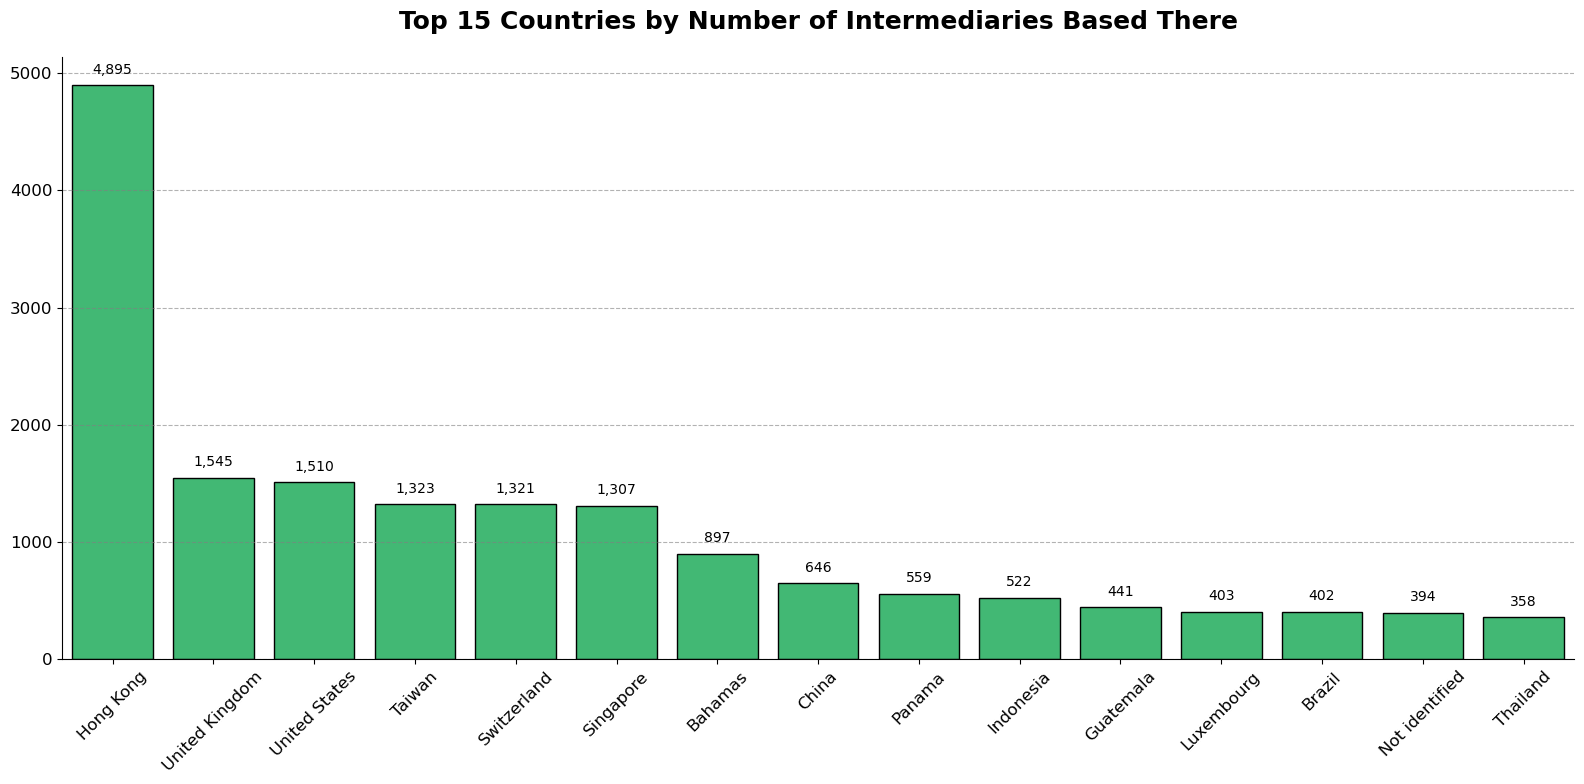
\includegraphics[width=0.8\textwidth]{intermediarieslocationsdesc.png}
    \caption{Geographic Distribution of Intermediaries (Top Locations).}
    \label{fig:int_locations}
\end{figure}

\begin{figure}[htbp]
    \centering
    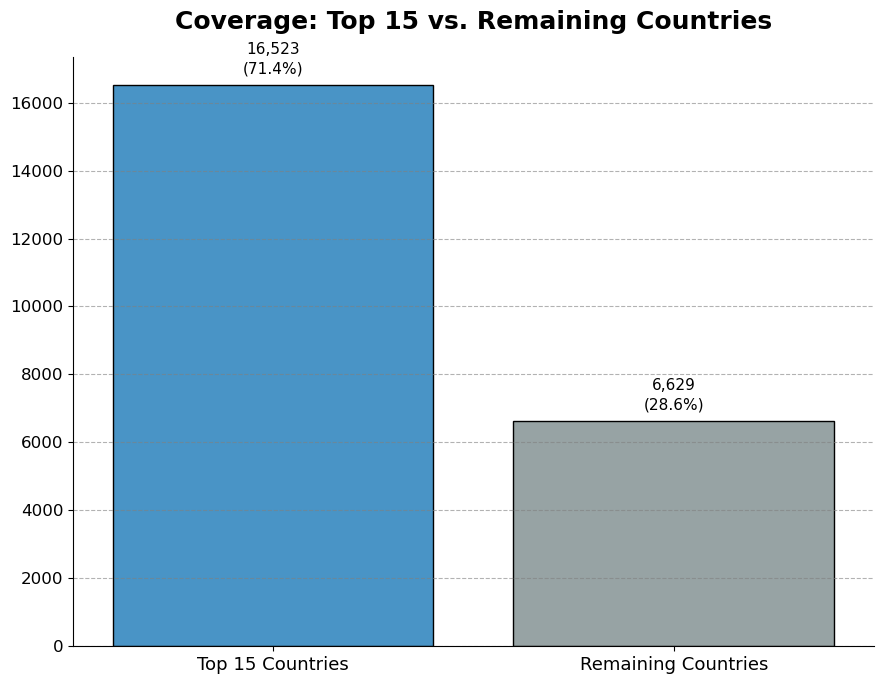
\includegraphics[width=0.8\textwidth]{intermediariescoverage.png}
    \caption{Coverage of Intermediaries by Top Geographic Locations.}
    \label{fig:int_coverage}
\end{figure}

\begin{figure}[htbp]
    \centering
    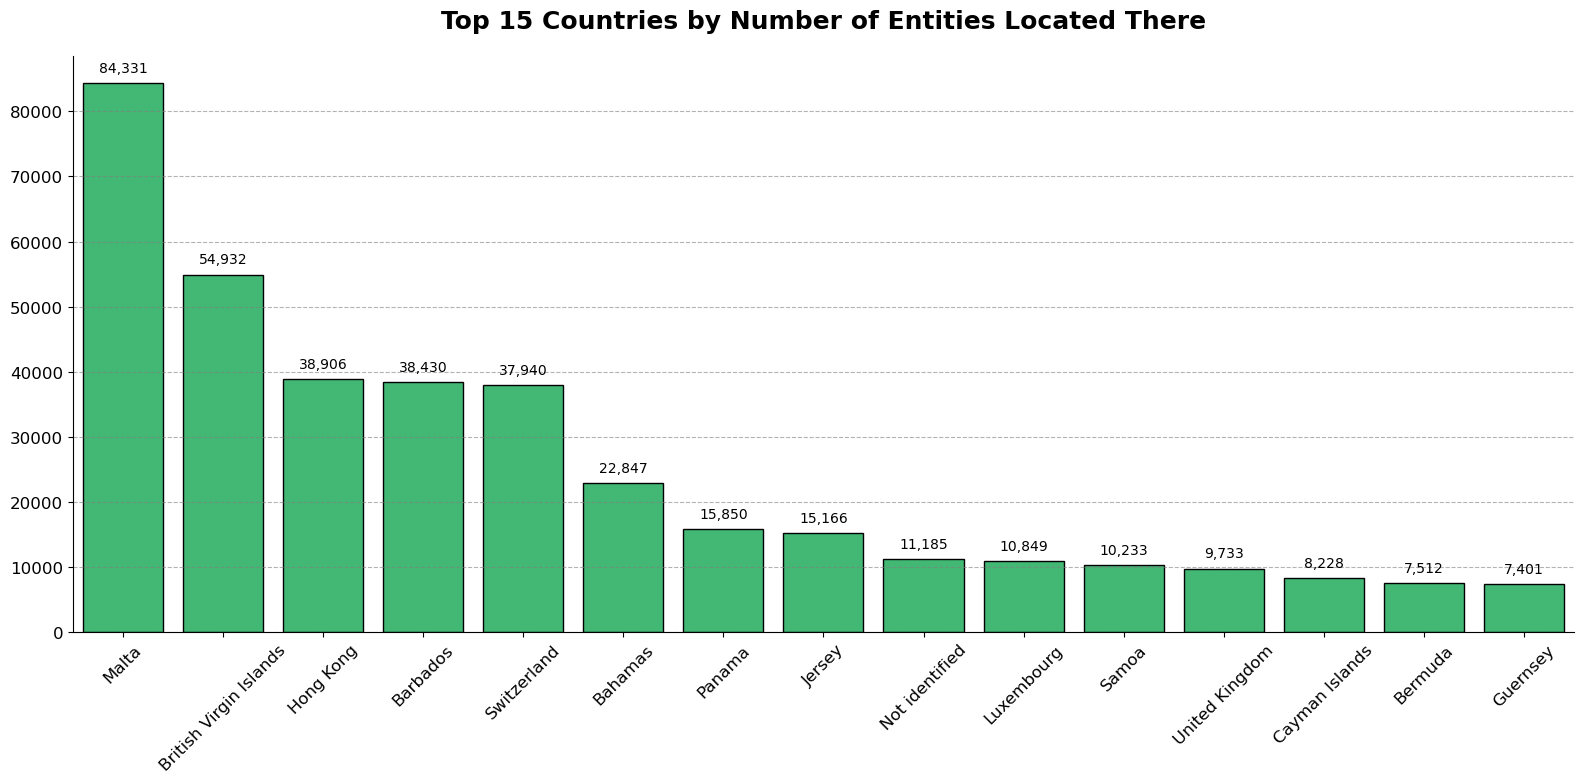
\includegraphics[width=0.8\textwidth]{entitieslocations.png}
    \caption{Geographic Distribution of Entities (Top Jurisdictions/Locations).}
    \label{fig:ent_locations}
\end{figure}

\begin{figure}[htbp]
    \centering
    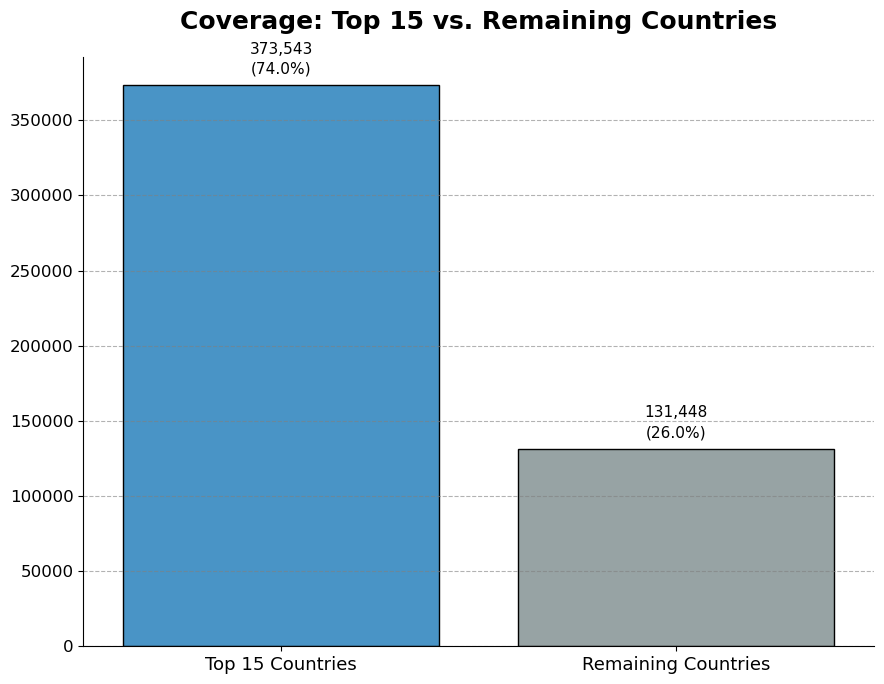
\includegraphics[width=0.8\textwidth]{entitiescoverage.png}
    \caption{Coverage of Entities by Top Geographic Locations.}
    \label{fig:ent_coverage}
\end{figure}

\begin{figure}[htbp]
    \centering
    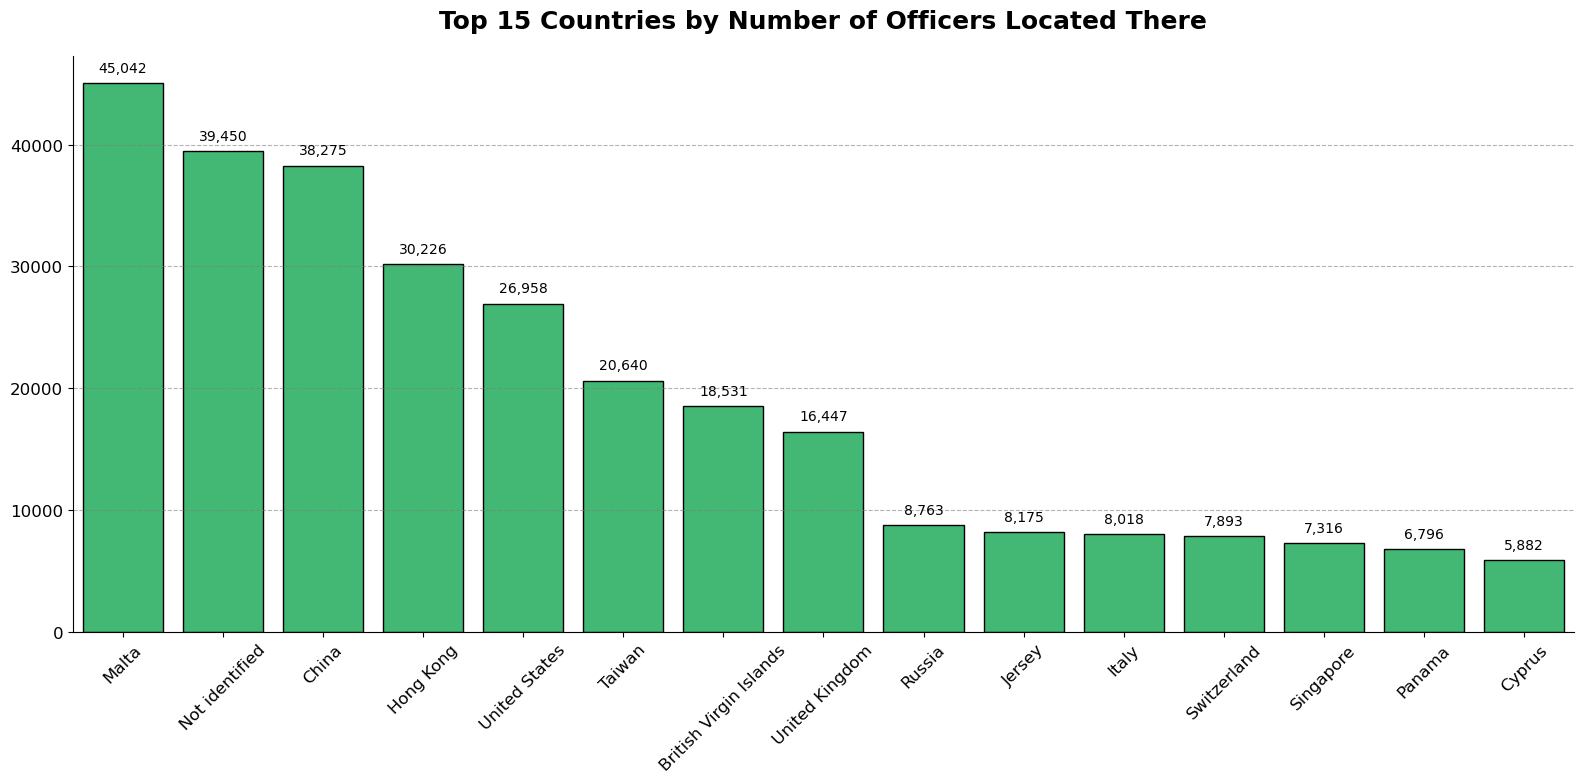
\includegraphics[width=0.8\textwidth]{officerslocation.png}
    \caption{Geographic Distribution of Officers (Top Locations).}
    \label{fig:off_locations}
\end{figure}

\begin{figure}[htbp]
    \centering
    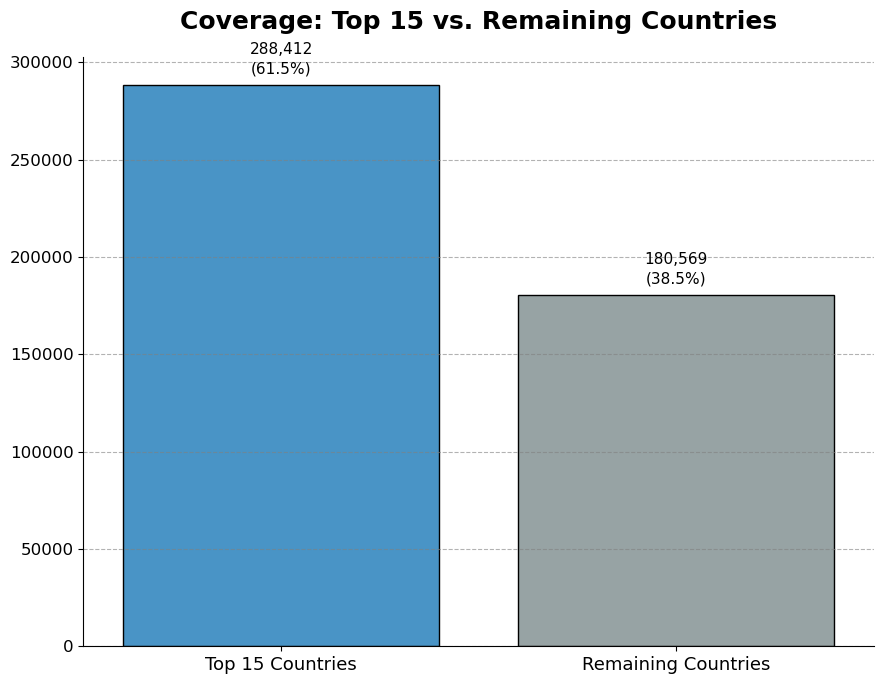
\includegraphics[width=0.8\textwidth]{officerscoverage.png}
    \caption{Coverage of Officers by Top Geographic Locations.}
    \label{fig:off_coverage}
\end{figure}

The enrichment process involved classifying intermediaries based on their likely role (e.g., Administrator, Legal Expert). Figure \ref{fig:classification_samples} compares the distribution of these classifications within the random sample versus the sample of top 5\% intermediaries.

\begin{figure}[htbp]
    \centering
    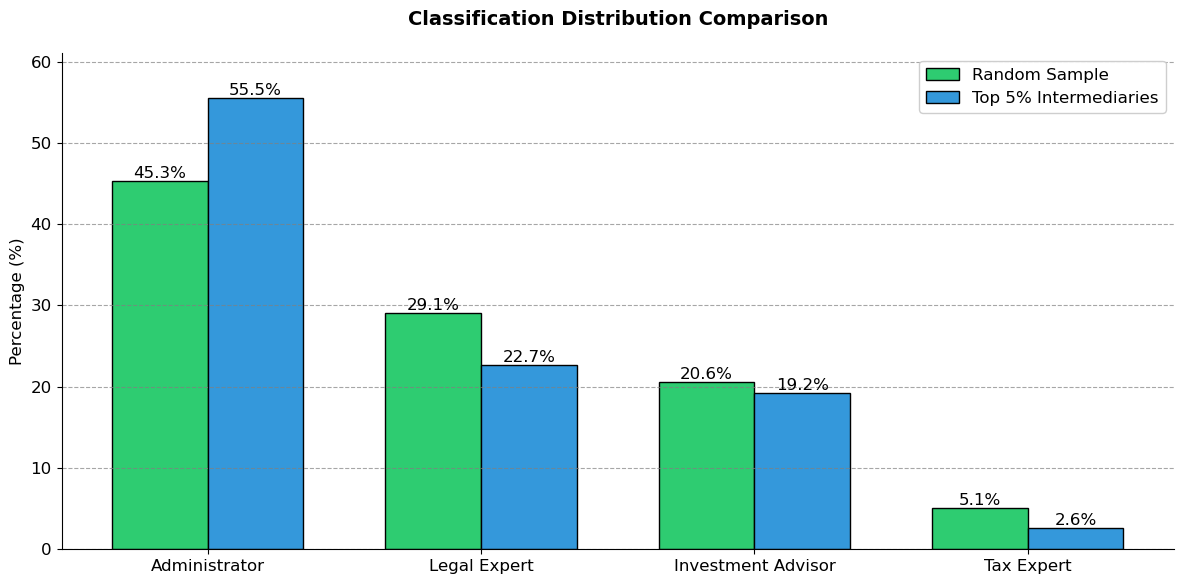
\includegraphics[width=0.8\textwidth]{classificationsamples.png}
    \caption{Comparison of Intermediary Classification Distributions (Random Sample vs. Top 5\%).}
    \label{fig:classification_samples}
\end{figure}

We observe distinct degree distributions based on these classifications. Figure \ref{fig:cdf_classifications} shows the Cumulative Distribution Function (CDF) of intermediary degrees for each classification, while Figure \ref{fig:boxplot_classifications} presents this comparison using boxplots.

\begin{figure}[htbp]
    \centering
    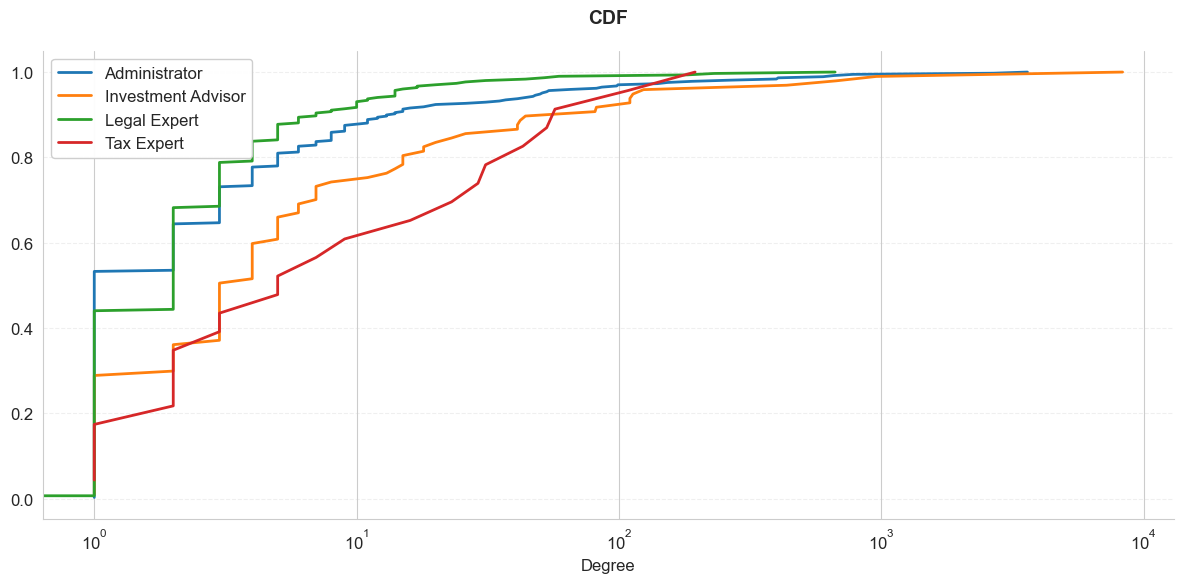
\includegraphics[width=0.8\textwidth]{CDFclassifications.png}
    \caption{Cumulative Distribution Function (CDF) of Intermediary Degree by Classification.}
    \label{fig:cdf_classifications}
\end{figure}

\begin{figure}[htbp]
    \centering
    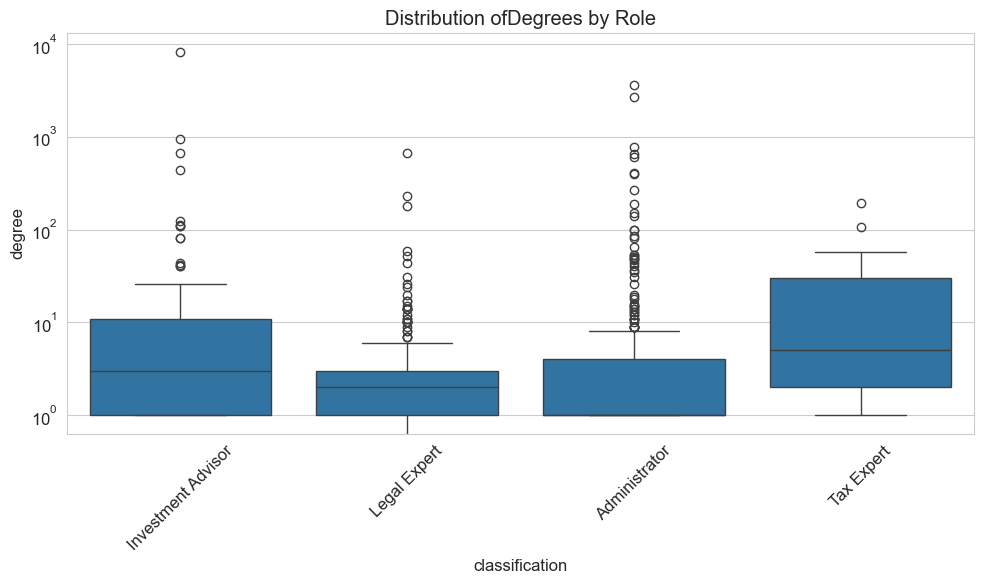
\includegraphics[width=0.8\textwidth]{boxplotclassification.png}
    \caption{Boxplot of Intermediary Degree by Classification.}
    \label{fig:boxplot_classifications}
\end{figure}

These classification patterns also vary geographically, as illustrated in Figure \ref{fig:countries_classifications}, which likely shows the prevalence of different intermediary types across key countries.

\begin{figure}[htbp]
    \centering
    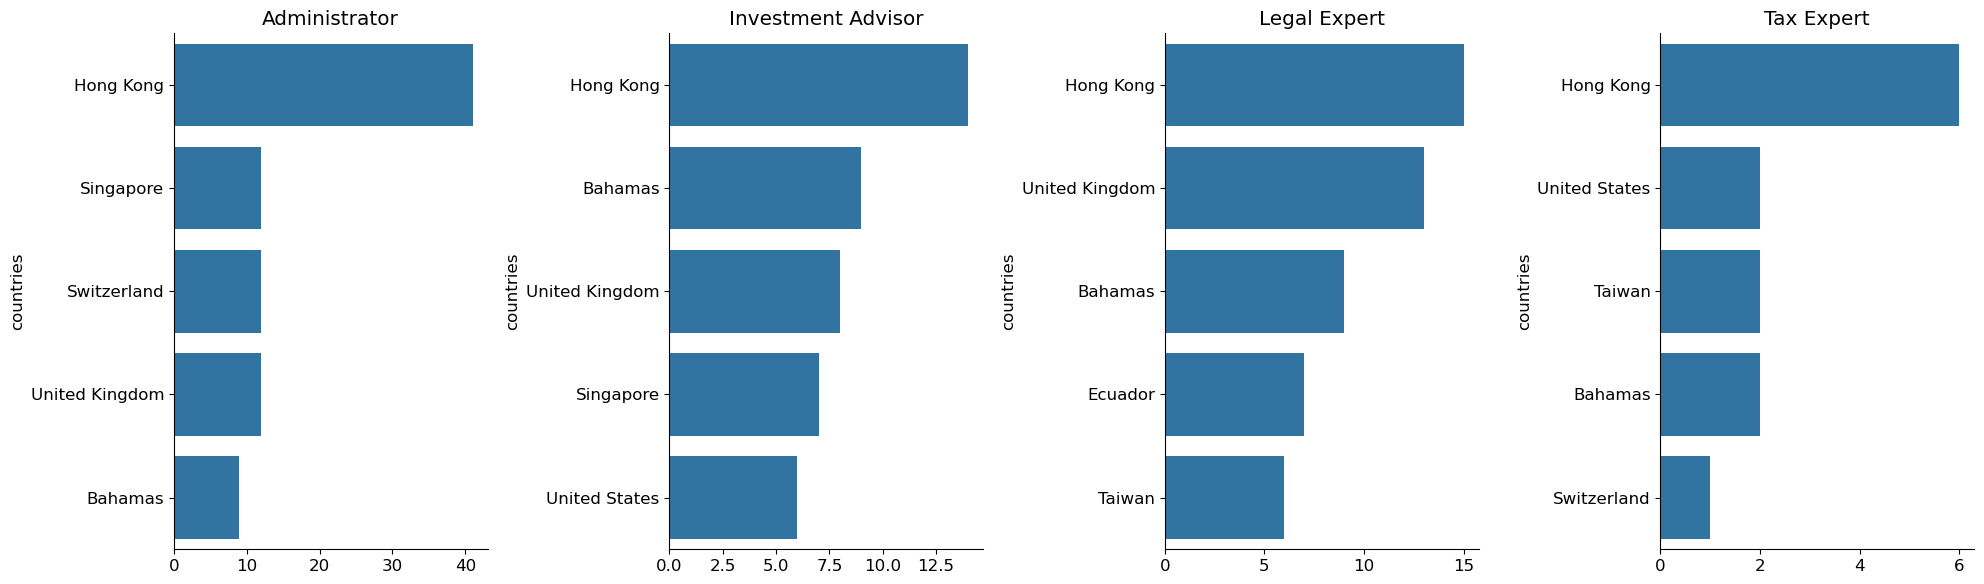
\includegraphics[width=0.8\textwidth]{countriesclassification.png}
    \caption{Distribution of Intermediary Classifications across Top Countries.}
    \label{fig:countries_classifications}
\end{figure}

Also, differing degree distributions, tested signifiance for.

Using a Negative Binomial GLM; cannot use Poisson because of overdispersion. 

Basic setup:

\textbf{Random Component:} The response $Y_i$ (degree of intermediary $i$) follows a Negative Binomial distribution, $Y_i \sim \text{NB}(\mu_i, \theta)$, accommodating count data with overdispersion where $\text{Var}(Y_i) = \mu_i + \mu_i^2 / \theta$.

\textbf{Link Function:} The expected value $\mu_i = E[Y_i]$ is related to the linear predictor $\eta_i = \mathbf{x}_i^T \boldsymbol{\beta}$ via the \textbf{natural logarithm} link function:
\[
    \ln(\mu_i) = \eta_i \quad \implies \quad \mu_i = \exp(\mathbf{x}_i^T \boldsymbol{\beta})
\]
where $\mathbf{x}_i$ includes dummy variables for the intermediary classification (with 'Administrator' likely as the baseline) and $\boldsymbol{\beta}$ are the coefficients to be estimated.

Since there is no closed-form solution for the parameters $\boldsymbol{\beta}$ and the dispersion parameter $\theta$, we numerically optimise the log-likelihood function:
\[
    \ell(\boldsymbol{\beta}, \theta) = \sum_{i=1}^n \ln \left[ P(Y_i=y_i | \mu_i = \exp(\mathbf{x}_i^T \boldsymbol{\beta}), \theta) \right]
\]

Results:
\begin{verbatim}
GLM Results (Negative Binomial):
                 Generalized Linear Model Regression Results                  
Dep. Variable:                 degree   No. Observations:                  790
Model:                            GLM   Df Residuals:                      786
Model Family:        NegativeBinomial   Df Model:                            3
Link Function:                    Log   Scale:                          1.0000
Method:                          IRLS   Log-Likelihood:                -3216.9
Date:                Mon, 12 May 2025   Deviance:                       2927.8
Time:                        13:00:11   Pearson chi2:                 3.51e+04
No. Iterations:                    12   Pseudo R-squ. (CS):             0.5825
Covariance Type:            nonrobust                                         
                                              coef    std err          z      P>|z|      [0.025      0.975]
-----------------------------------------------------------------------------------------------------------
Intercept                                   3.4632      0.053     65.419      0.000       3.359       3.567
C(classification)[T.Investment Advisor]     1.3162      0.115     11.457      0.000       1.091       1.541
C(classification)[T.Legal Expert]          -1.5206      0.081    -18.734      0.000      -1.680      -1.362
C(classification)[T.Tax Expert]            -0.2034      0.219     -0.929      0.353      -0.633       0.226
\end{verbatim}

The GLM results indicate significant differences in degree based on classification. Compared to the baseline (likely 'Administrator'), 'Investment Advisor' intermediaries have significantly higher degrees, while 'Legal Expert' intermediaries have significantly lower degrees. The 'Tax Expert' classification does not show a statistically significant difference from the baseline in this model. These findings are further corroborated by an Ordinary Least Squares (OLS) regression using the logarithm of the degree ($\log(\text{degree})$) as the target variable (results not shown here but confirm the direction and significance of the effects).


While static comparisons are (moderately) informative, the temporal progress of the network structure offers more dynamic insights. Figure \ref{fig:cyprus_temporal} presents a case study focused on Cyprus, illustrating how the connections between different types of intermediaries and the locations (jurisdictions/countries) of the entities they service evolve over time.

Starting with all intermediaries from Cyprus, and then grouping entities together based on where they are 1) based in terms of business activity (`countries` field provided by ICIJ) and the jurisdiction whose rules they follow (`jurisdiction` field provided by ICIJ)

Two things to note:
\begin{enumerate}
    \item Corroborates the well-documented picture of a gradually deepening network tied to Russia, as more and more entities connected to it, and 
    \item Primary intermediaries that are first needed are Administrators, and then more peripheral intermediary roles become involved (e.g., Legal Experts, Tax Experts). Too sparse to conclude it from this case study alone, but consistent with the idea that the network starts with a core of essential roles and then expands to include more specialized functions as the network grows.
\end{enumerate}
\begin{figure}[htbp]
    \centering
    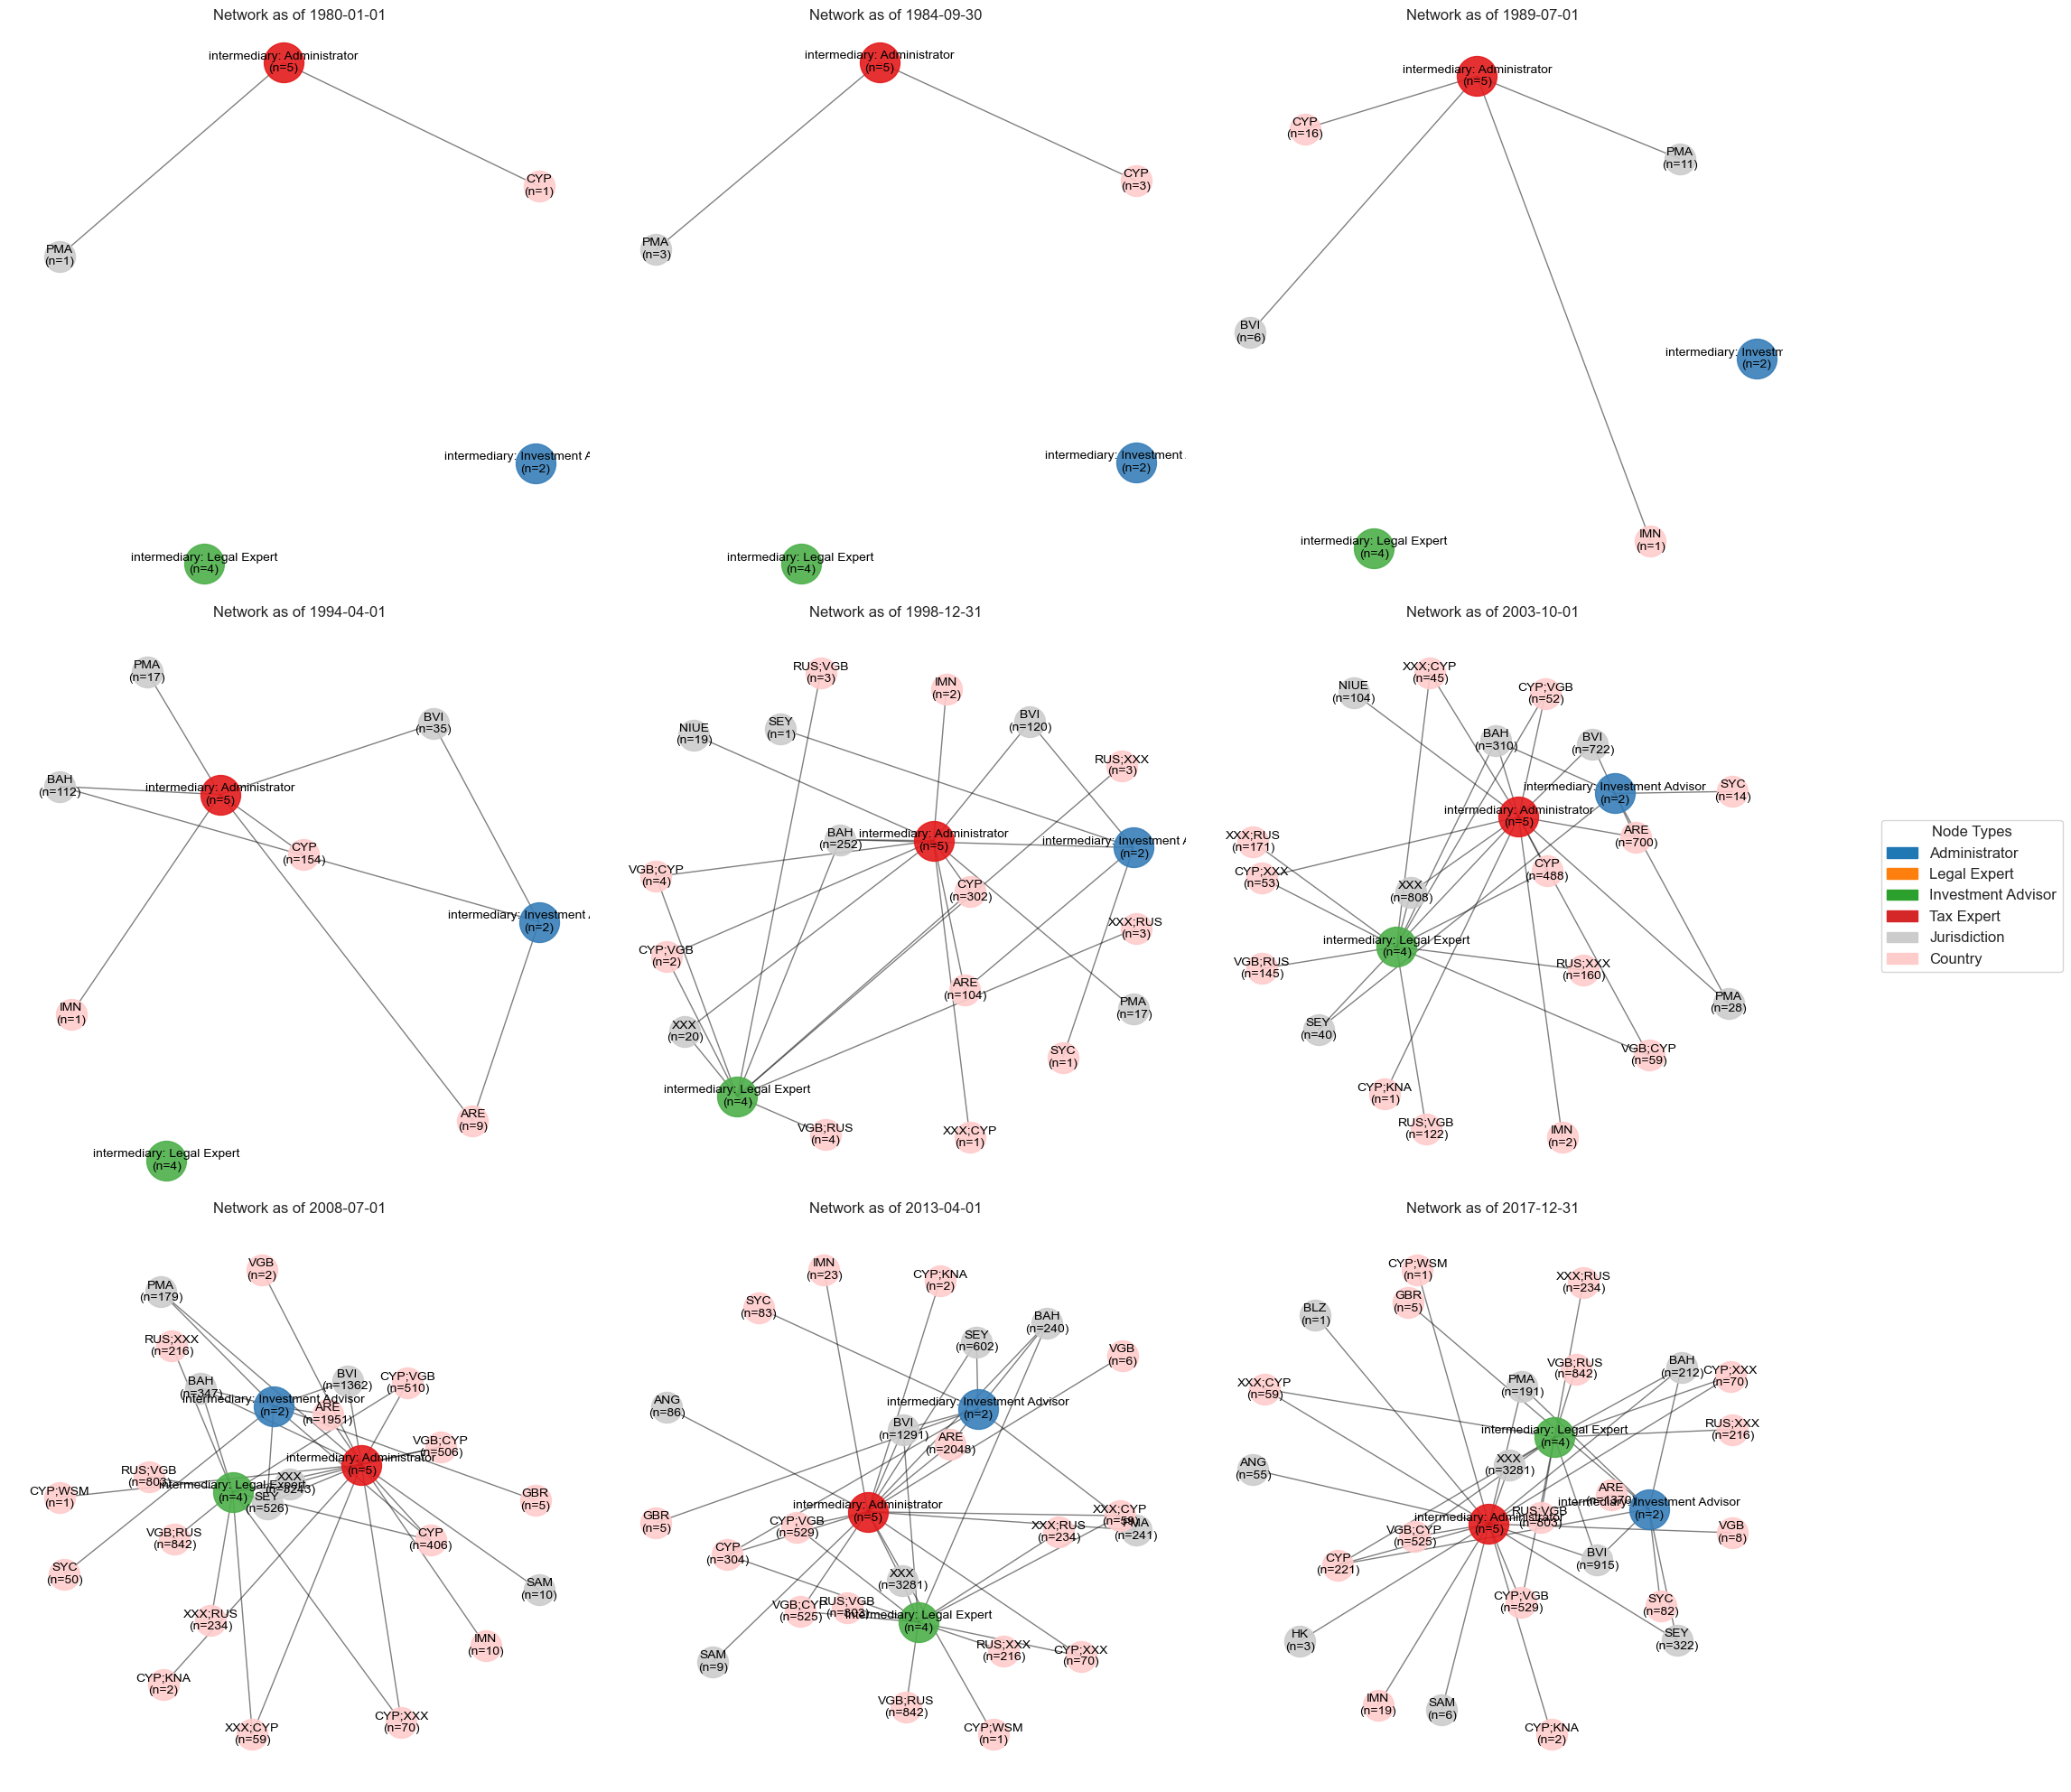
\includegraphics[width=0.9\textwidth]{CyprusCaseStudy.png} 
    \caption{Temporal Evolution of the Intermediary-Entity Network (Cyprus Case Study). Shows connections between intermediary types (based in Cyprus) and the locations of entities they manage at different time points.}
    \label{fig:cyprus_temporal}
\end{figure}


